\documentclass{article}
\usepackage{tikz}
\begin{document}
	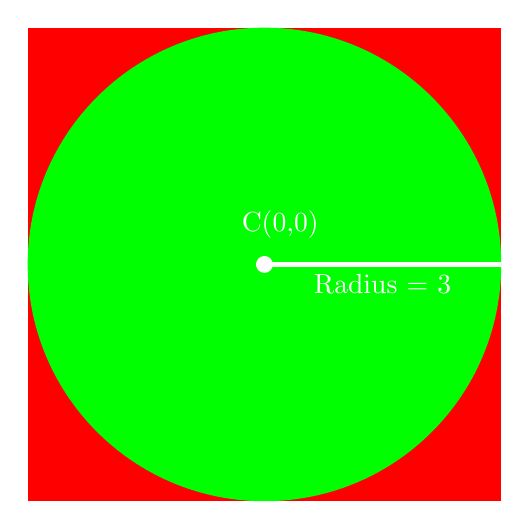
\begin{tikzpicture}
		%\draw[fill,red] (0,0) -- (1,0);
		\draw[fill,red] (-3,-3) rectangle(3,3);
		\draw[fill,green] (0,0) circle[radius = 3];
		\draw[fill,white] (0,0) circle[radius = 0.1];
		\draw[ultra thick,fill,white] (0,0) -- (3,0);
		\node[white] at (0.2,0.5) {C(0,0)};
		\node[below,white] at (1.5,0) {Radius = 3};
		%\node[above] at (0,0) {Radius = 3};
	\end{tikzpicture}
\end{document}